\documentclass[11pt,a4paper]{article}
\usepackage[latin1]{inputenc}
\usepackage{amsmath}
\usepackage{amsfonts}
\usepackage{amssymb}
\usepackage{graphicx}
\usepackage{float}
\usepackage{fancyhdr}
\fancyhead[L]{MovieMatcher User Guide}
\fancyhead[R]{April 6, 2016}
\pagestyle{fancy}
\date{April 6, 2016}
\author{Chowdhry, Bilal 1320763\\
Hu, Joshua 1311940\\
Kapinski, Justin 1305257\\
Lakdawala, Shaad 1335602\\
Muhammad, Abdullah 1317053\\
Patel, Keyur 1311559}
\title{MovieMatcher User Guide}
\begin{document}
\clearpage
\maketitle
\thispagestyle{empty}
\newpage

\section{Introduction}
This guide is intended to inform the user on the purpose and intended method of interaction with the MovieMatcher application.\\
\\
MovieMatcher is a recommendation application that tells the user of this application what movie best matches the criteria of their search. It also suggests alternatives that may also be the movie they are looking for. As an additional feature they can choose to view the shooting locations of a movie on a map interface.

\section{Use}
Each expert has a certain weight factor to their response, and a cumulative result is determined based on the 3 experts' results.\\
\\
3 Fields inside the app, one for each expert
\begin{itemize}
\item[First Expert:] enter names in one line, separated by commas (eg. Christian Bale)
\item[Second Expert:] Enter genre and keywords in one line, separated by commas (eg. Action)
\item[Third Expert:] Enter the quotes in one line, separated by semicolons (eg. Why so serious)
\end{itemize}

\begin{figure}[H]
\centering
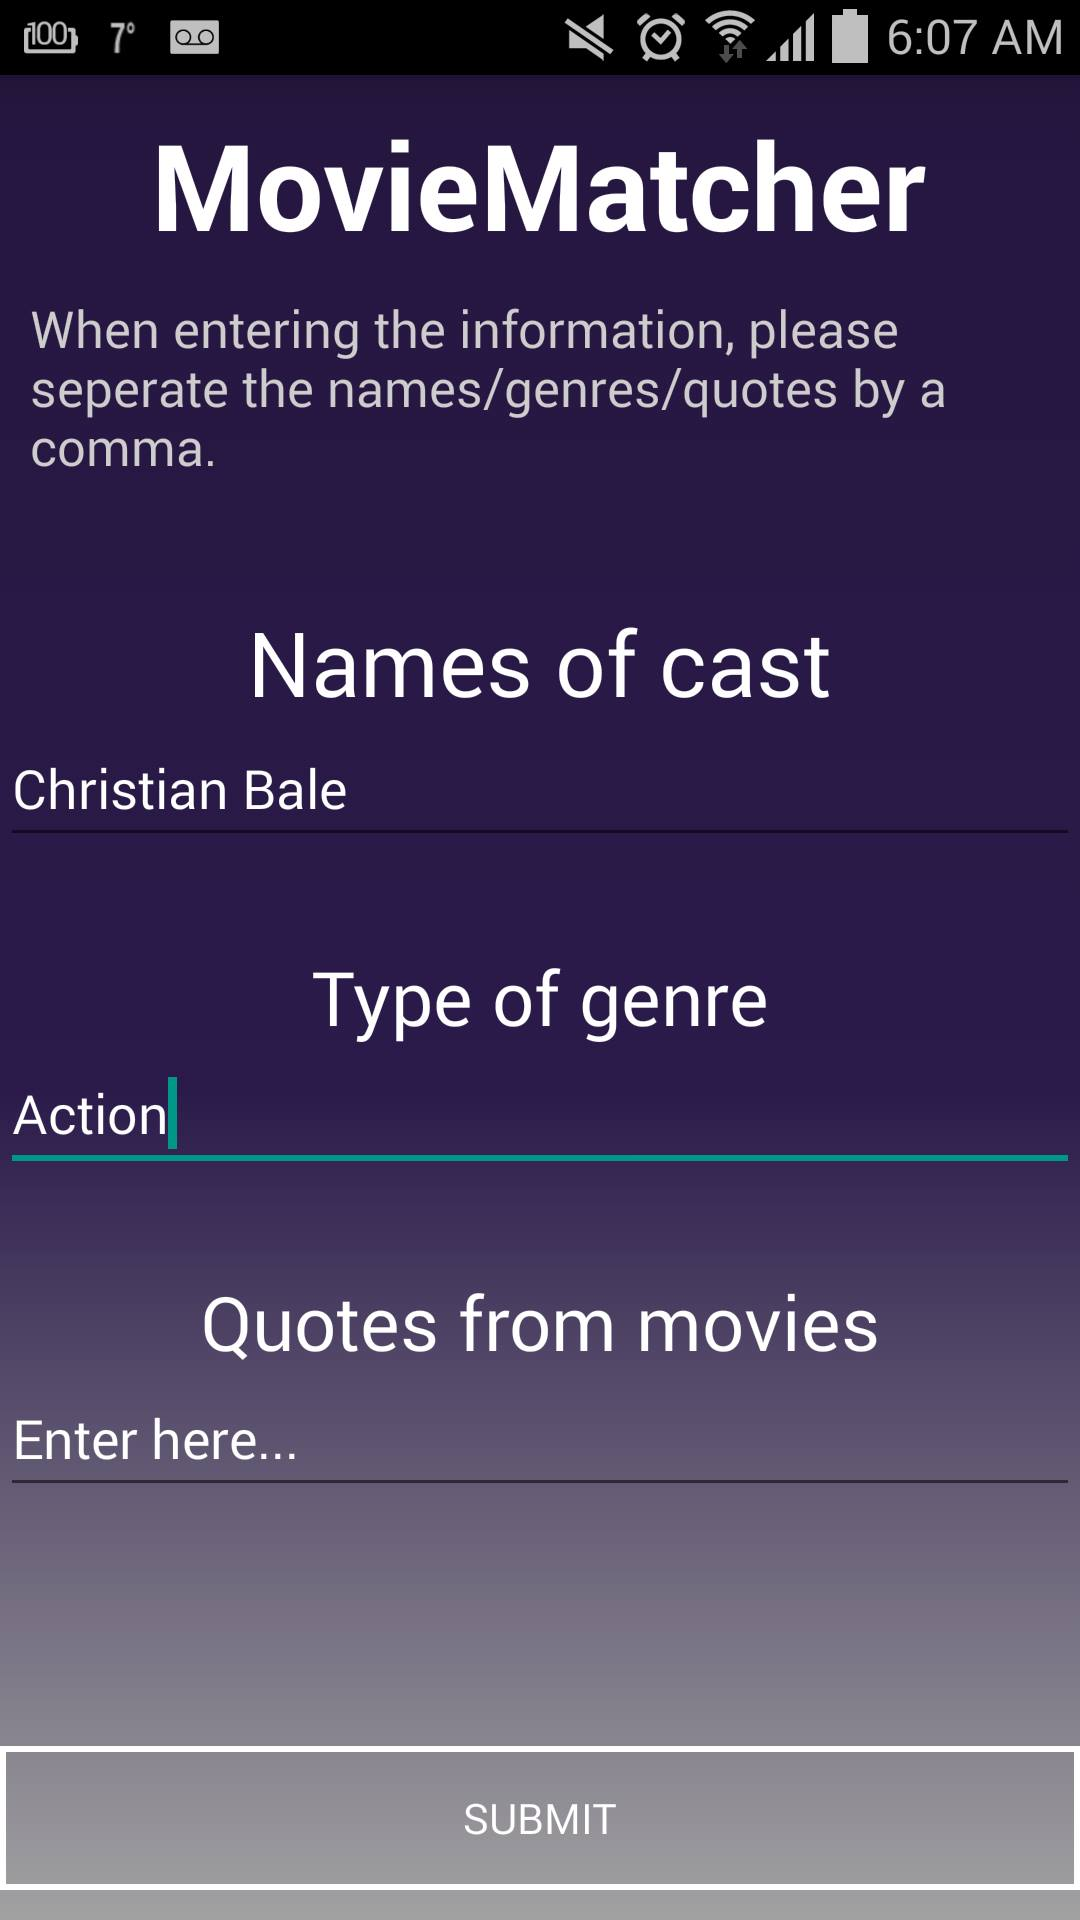
\includegraphics[scale=.08]{screen1.jpg}
\caption{The search screen}
\end{figure}

Click the submit button to process your information and view the results.\\
\\

On the results page:
\begin{itemize}
\item[] Top result is the best result based on your provided information
\item[] Next 2 results are the other experts' results (may be the same, or different)
\end{itemize}

\begin{figure}[H]
\centering
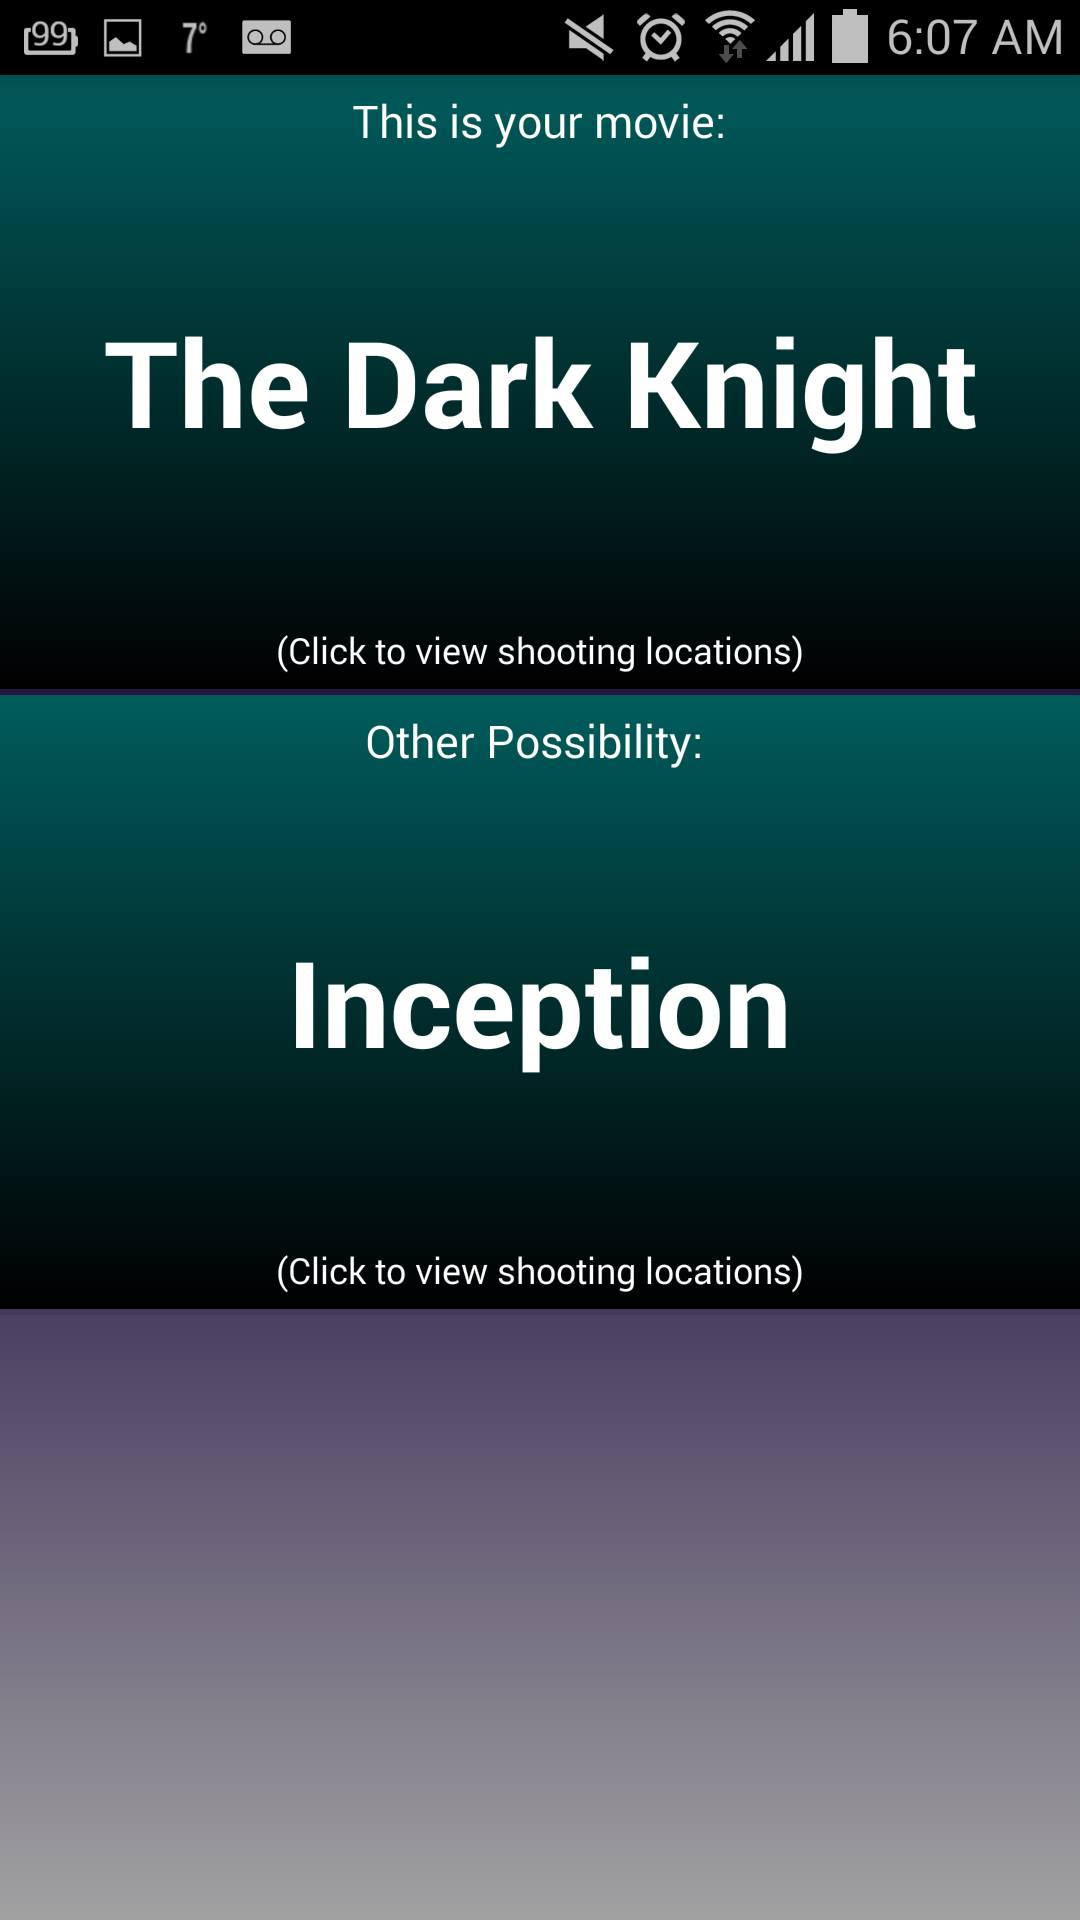
\includegraphics[scale=.08]{screen2.jpg}
\caption{The search screen}
\end{figure} 

To view the shooting locations of any of the results, simply click on the movie for which you would like to see the locations, and MovieMatcher will present you with a Google Maps view with the filming locations highlighted with markers.\\

\begin{figure}[H]
\centering
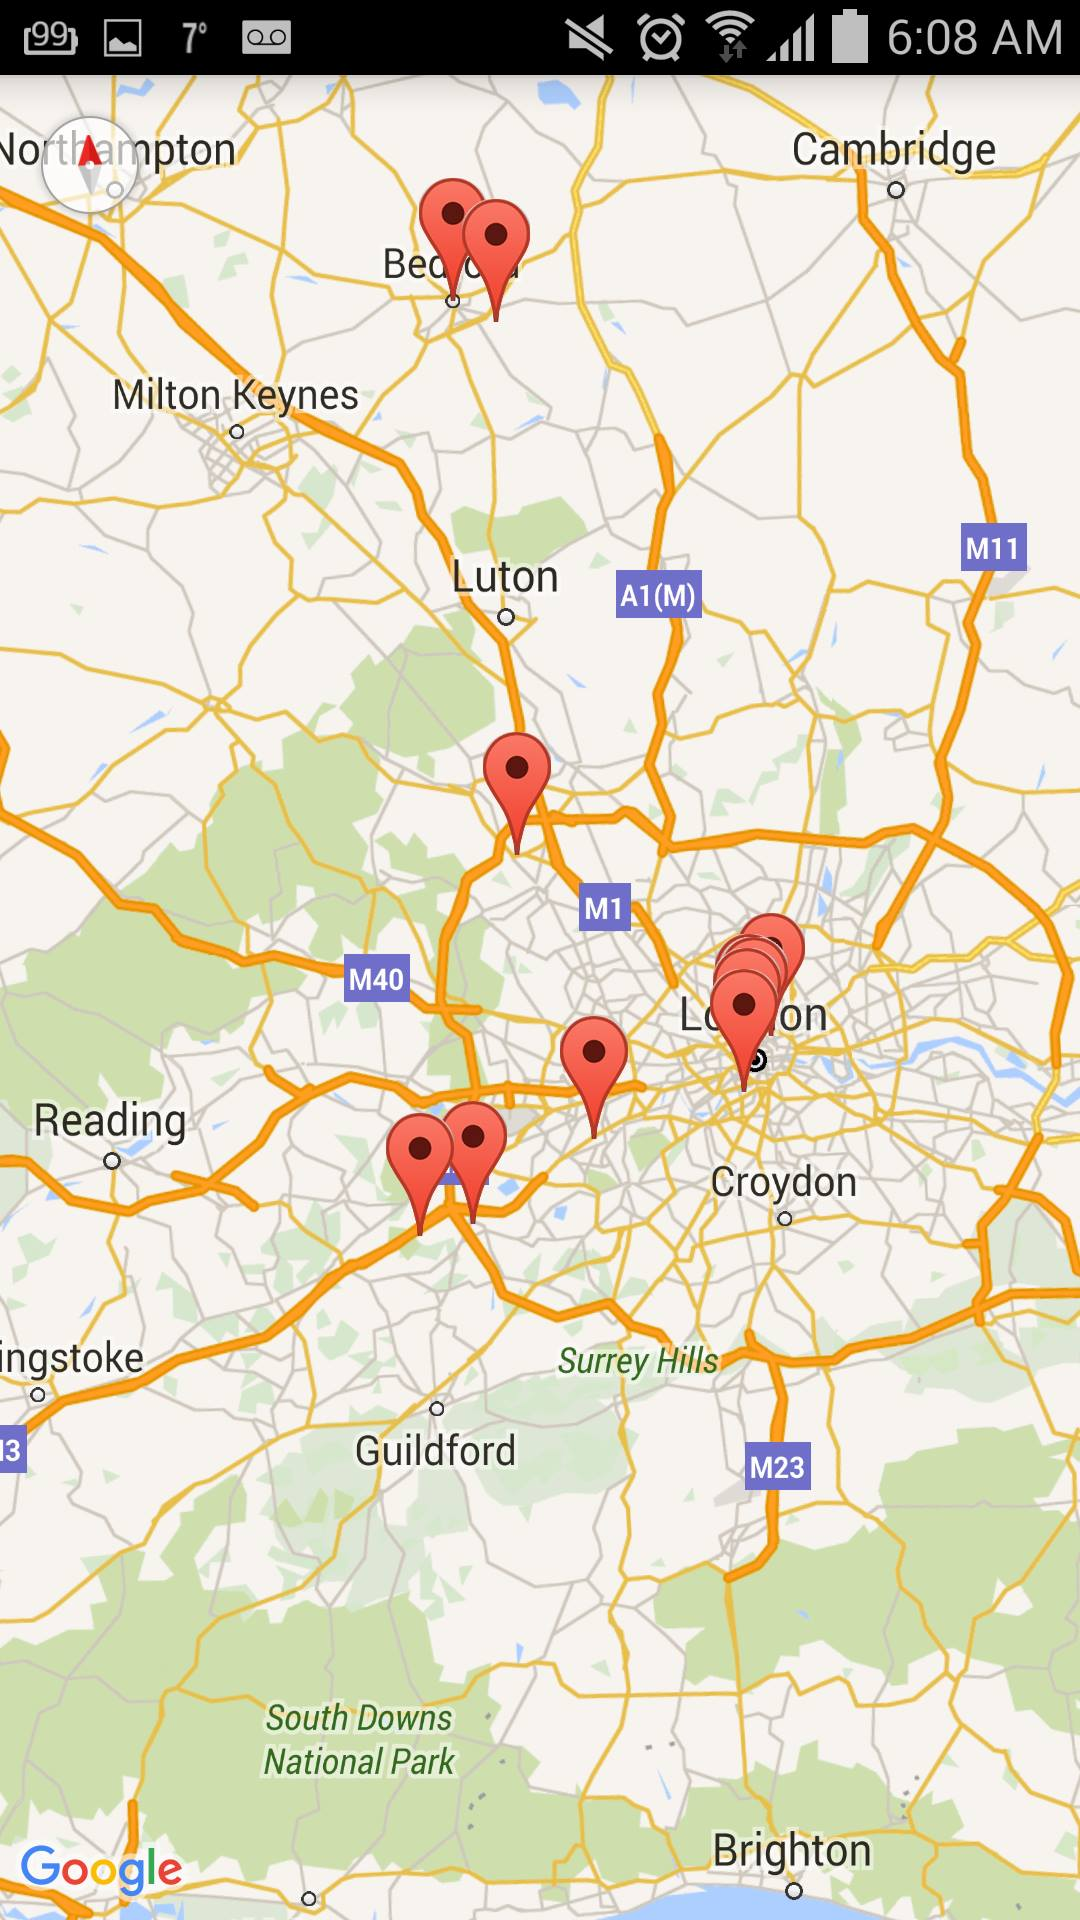
\includegraphics[scale=.08]{screen3.jpg}
\caption{The search screen}
\end{figure}

\end{document}